\documentclass[twoside]{book}

% Packages required by doxygen
\usepackage{fixltx2e}
\usepackage{calc}
\usepackage{doxygen}
\usepackage[export]{adjustbox} % also loads graphicx
\usepackage{graphicx}
\usepackage[utf8]{inputenc}
\usepackage{makeidx}
\usepackage{multicol}
\usepackage{multirow}
\PassOptionsToPackage{warn}{textcomp}
\usepackage{textcomp}
\usepackage[nointegrals]{wasysym}
\usepackage[table]{xcolor}

% Font selection
\usepackage[T1]{fontenc}
\usepackage[scaled=.90]{helvet}
\usepackage{courier}
\usepackage{amssymb}
\usepackage{sectsty}
\renewcommand{\familydefault}{\sfdefault}
\allsectionsfont{%
  \fontseries{bc}\selectfont%
  \color{darkgray}%
}
\renewcommand{\DoxyLabelFont}{%
  \fontseries{bc}\selectfont%
  \color{darkgray}%
}
\newcommand{\+}{\discretionary{\mbox{\scriptsize$\hookleftarrow$}}{}{}}

% Page & text layout
\usepackage{geometry}
\geometry{%
  a4paper,%
  top=2.5cm,%
  bottom=2.5cm,%
  left=2.5cm,%
  right=2.5cm%
}
\tolerance=750
\hfuzz=15pt
\hbadness=750
\setlength{\emergencystretch}{15pt}
\setlength{\parindent}{0cm}
\setlength{\parskip}{3ex plus 2ex minus 2ex}
\makeatletter
\renewcommand{\paragraph}{%
  \@startsection{paragraph}{4}{0ex}{-1.0ex}{1.0ex}{%
    \normalfont\normalsize\bfseries\SS@parafont%
  }%
}
\renewcommand{\subparagraph}{%
  \@startsection{subparagraph}{5}{0ex}{-1.0ex}{1.0ex}{%
    \normalfont\normalsize\bfseries\SS@subparafont%
  }%
}
\makeatother

% Headers & footers
\usepackage{fancyhdr}
\pagestyle{fancyplain}
\fancyhead[LE]{\fancyplain{}{\bfseries\thepage}}
\fancyhead[CE]{\fancyplain{}{}}
\fancyhead[RE]{\fancyplain{}{\bfseries\leftmark}}
\fancyhead[LO]{\fancyplain{}{\bfseries\rightmark}}
\fancyhead[CO]{\fancyplain{}{}}
\fancyhead[RO]{\fancyplain{}{\bfseries\thepage}}
\fancyfoot[LE]{\fancyplain{}{}}
\fancyfoot[CE]{\fancyplain{}{}}
\fancyfoot[RE]{\fancyplain{}{\bfseries\scriptsize Generated by Doxygen }}
\fancyfoot[LO]{\fancyplain{}{\bfseries\scriptsize Generated by Doxygen }}
\fancyfoot[CO]{\fancyplain{}{}}
\fancyfoot[RO]{\fancyplain{}{}}
\renewcommand{\footrulewidth}{0.4pt}
\renewcommand{\chaptermark}[1]{%
  \markboth{#1}{}%
}
\renewcommand{\sectionmark}[1]{%
  \markright{\thesection\ #1}%
}

% Indices & bibliography
\usepackage{natbib}
\usepackage[titles]{tocloft}
\setcounter{tocdepth}{3}
\setcounter{secnumdepth}{5}
\makeindex

% Hyperlinks (required, but should be loaded last)
\usepackage{ifpdf}
\ifpdf
  \usepackage[pdftex,pagebackref=true]{hyperref}
\else
  \usepackage[ps2pdf,pagebackref=true]{hyperref}
\fi
\hypersetup{%
  colorlinks=true,%
  linkcolor=blue,%
  citecolor=blue,%
  unicode%
}

% Custom commands
\newcommand{\clearemptydoublepage}{%
  \newpage{\pagestyle{empty}\cleardoublepage}%
}

\usepackage{caption}
\captionsetup{labelsep=space,justification=centering,font={bf},singlelinecheck=off,skip=4pt,position=top}

%===== C O N T E N T S =====

\begin{document}

% Titlepage & ToC
\hypersetup{pageanchor=false,
             bookmarksnumbered=true,
             pdfencoding=unicode
            }
\pagenumbering{alph}
\begin{titlepage}
\vspace*{7cm}
\begin{center}%
{\Large A\+C\+ME Perception }\\
\vspace*{1cm}
{\large Generated by Doxygen 1.8.13}\\
\end{center}
\end{titlepage}
\clearemptydoublepage
\pagenumbering{roman}
\tableofcontents
\clearemptydoublepage
\pagenumbering{arabic}
\hypersetup{pageanchor=true}

%--- Begin generated contents ---
\chapter{Namespace Index}
\section{Namespace List}
Here is a list of all namespaces with brief descriptions\+:\begin{DoxyCompactList}
\item\contentsline{section}{\hyperlink{namespaceall__params}{all\+\_\+params} }{\pageref{namespaceall__params}}{}
\end{DoxyCompactList}

\chapter{Hierarchical Index}
\section{Class Hierarchy}
This inheritance list is sorted roughly, but not completely, alphabetically\+:\begin{DoxyCompactList}
\item \contentsline{section}{Detection}{\pageref{struct_detection}}{}
\item exception\begin{DoxyCompactList}
\item \contentsline{section}{Invalid\+File}{\pageref{class_invalid_file}}{}
\end{DoxyCompactList}
\item \contentsline{section}{Human\+Detector}{\pageref{class_human_detector}}{}
\item \contentsline{section}{Label\+Parser}{\pageref{class_label_parser}}{}
\item \contentsline{section}{Param\+Parser}{\pageref{class_param_parser}}{}
\item \contentsline{section}{Position\+Estimator}{\pageref{class_position_estimator}}{}
\item \contentsline{section}{Test\+Image}{\pageref{struct_test_image}}{}
\item \contentsline{section}{Var}{\pageref{struct_var}}{}
\item \contentsline{section}{Vision\+A\+PI}{\pageref{class_vision_a_p_i}}{}
\end{DoxyCompactList}

\chapter{Class Index}
\section{Class List}
Here are the classes, structs, unions and interfaces with brief descriptions\+:\begin{DoxyCompactList}
\item\contentsline{section}{\hyperlink{struct_detection}{Detection} \\*This struct will be used to pass detection information between the human detector and position estimator classes. See the U\+ML for more information }{\pageref{struct_detection}}{}
\item\contentsline{section}{\hyperlink{class_human_detector}{Human\+Detector} }{\pageref{class_human_detector}}{}
\item\contentsline{section}{\hyperlink{class_param_parser}{Param\+Parser} }{\pageref{class_param_parser}}{}
\item\contentsline{section}{\hyperlink{class_position_estimator}{Position\+Estimator} }{\pageref{class_position_estimator}}{}
\item\contentsline{section}{\hyperlink{struct_var}{Var} }{\pageref{struct_var}}{}
\item\contentsline{section}{\hyperlink{class_vision_a_p_i}{Vision\+A\+PI} }{\pageref{class_vision_a_p_i}}{}
\end{DoxyCompactList}

\chapter{File Index}
\section{File List}
Here is a list of all files with brief descriptions\+:\begin{DoxyCompactList}
\item\contentsline{section}{/media/diane/\+My Passport/\+U\+M\+D Masters/\+Fall 2021/\+E\+N\+P\+M 808\+X/\+Assignments/\+Midterm/\+A\+C\+M\+E\+\_\+perception\+\_\+proposal/include/\hyperlink{_detection_8hpp}{Detection.\+hpp} }{\pageref{_detection_8hpp}}{}
\item\contentsline{section}{/media/diane/\+My Passport/\+U\+M\+D Masters/\+Fall 2021/\+E\+N\+P\+M 808\+X/\+Assignments/\+Midterm/\+A\+C\+M\+E\+\_\+perception\+\_\+proposal/include/\hyperlink{_human_detector_8hpp}{Human\+Detector.\+hpp} }{\pageref{_human_detector_8hpp}}{}
\item\contentsline{section}{/media/diane/\+My Passport/\+U\+M\+D Masters/\+Fall 2021/\+E\+N\+P\+M 808\+X/\+Assignments/\+Midterm/\+A\+C\+M\+E\+\_\+perception\+\_\+proposal/include/\hyperlink{_param_parser_8hpp}{Param\+Parser.\+hpp} }{\pageref{_param_parser_8hpp}}{}
\item\contentsline{section}{/media/diane/\+My Passport/\+U\+M\+D Masters/\+Fall 2021/\+E\+N\+P\+M 808\+X/\+Assignments/\+Midterm/\+A\+C\+M\+E\+\_\+perception\+\_\+proposal/include/\hyperlink{_position_estimator_8hpp}{Position\+Estimator.\+hpp} }{\pageref{_position_estimator_8hpp}}{}
\item\contentsline{section}{/media/diane/\+My Passport/\+U\+M\+D Masters/\+Fall 2021/\+E\+N\+P\+M 808\+X/\+Assignments/\+Midterm/\+A\+C\+M\+E\+\_\+perception\+\_\+proposal/include/\hyperlink{_vision_a_p_i_8hpp}{Vision\+A\+P\+I.\+hpp} }{\pageref{_vision_a_p_i_8hpp}}{}
\end{DoxyCompactList}

\chapter{Namespace Documentation}
\hypertarget{namespaceall__params}{}\section{all\+\_\+params Namespace Reference}
\label{namespaceall__params}\index{all\+\_\+params@{all\+\_\+params}}
\subsection*{Variables}
\begin{DoxyCompactItemize}
\item 
std\+::vector$<$ \hyperlink{struct_var}{Var} $>$ \hyperlink{namespaceall__params_a925d27c82562242237a980dc8c86bc4a}{params}
\end{DoxyCompactItemize}


\subsection{Variable Documentation}
\mbox{\Hypertarget{namespaceall__params_a925d27c82562242237a980dc8c86bc4a}\label{namespaceall__params_a925d27c82562242237a980dc8c86bc4a}} 
\index{all\+\_\+params@{all\+\_\+params}!params@{params}}
\index{params@{params}!all\+\_\+params@{all\+\_\+params}}
\subsubsection{\texorpdfstring{params}{params}}
{\footnotesize\ttfamily std\+::vector$<$\hyperlink{struct_var}{Var}$>$ all\+\_\+params\+::params}


\chapter{Class Documentation}
\hypertarget{struct_detection}{}\section{Detection Struct Reference}
\label{struct_detection}\index{Detection@{Detection}}


This struct will be used to pass detection information between the human detector and position estimator classes. See the U\+ML for more information.  




{\ttfamily \#include $<$Detection.\+hpp$>$}

\subsection*{Public Member Functions}
\begin{DoxyCompactItemize}
\item 
\hyperlink{struct_detection}{Detection} \& \hyperlink{struct_detection_a98d5bca326ea2f369156fb07be1f5466}{operator=} (const \hyperlink{struct_detection}{Detection} \&detect)
\item 
\hyperlink{struct_detection}{Detection} \hyperlink{struct_detection_a69eb856cdc75d10db04c169d557815d1}{operator+} (const \hyperlink{struct_detection}{Detection} \&detect) const
\item 
\hyperlink{struct_detection}{Detection} \hyperlink{struct_detection_ae156f11b8c51921c6c785a921fc43e85}{operator-\/} (const \hyperlink{struct_detection}{Detection} \&detect) const
\item 
\hyperlink{struct_detection}{Detection} \& \hyperlink{struct_detection_a51bbeca262f4c0328f85eb9b32e97020}{operator+=} (const \hyperlink{struct_detection}{Detection} \&detect)
\item 
\hyperlink{struct_detection_a86e6ebf5a660a29e78ee7a7f08292260}{Detection} ()
\item 
\hyperlink{struct_detection_ac35051436ab3ae544f40f9aa08a0ebb1}{Detection} (int x\+\_\+, int y\+\_\+, int w, int h)
\item 
\hyperlink{struct_detection_ad50a7695ff3ce61ee5c10443d9210c1e}{Detection} (const \hyperlink{struct_detection}{Detection} \&detect)
\end{DoxyCompactItemize}
\subsection*{Public Attributes}
\begin{DoxyCompactItemize}
\item 
int \hyperlink{struct_detection_a7b71921325261514cd6dd42c8e90ba70}{x} \{0\}
\item 
int \hyperlink{struct_detection_afa5d065ea13ce74dfd52c6a569313270}{y} \{0\}
\item 
int \hyperlink{struct_detection_af88e469657d3bc4807caff6c5f9e9475}{width} \{0\}
\item 
int \hyperlink{struct_detection_a4f3d0bf4072f7e5a200767ab3d838fe2}{height} \{0\}
\end{DoxyCompactItemize}


\subsection{Detailed Description}
This struct will be used to pass detection information between the human detector and position estimator classes. See the U\+ML for more information. 

\subsection{Constructor \& Destructor Documentation}
\mbox{\Hypertarget{struct_detection_a86e6ebf5a660a29e78ee7a7f08292260}\label{struct_detection_a86e6ebf5a660a29e78ee7a7f08292260}} 
\index{Detection@{Detection}!Detection@{Detection}}
\index{Detection@{Detection}!Detection@{Detection}}
\subsubsection{\texorpdfstring{Detection()}{Detection()}\hspace{0.1cm}{\footnotesize\ttfamily [1/3]}}
{\footnotesize\ttfamily Detection\+::\+Detection (\begin{DoxyParamCaption}{ }\end{DoxyParamCaption})\hspace{0.3cm}{\ttfamily [inline]}}

\mbox{\Hypertarget{struct_detection_ac35051436ab3ae544f40f9aa08a0ebb1}\label{struct_detection_ac35051436ab3ae544f40f9aa08a0ebb1}} 
\index{Detection@{Detection}!Detection@{Detection}}
\index{Detection@{Detection}!Detection@{Detection}}
\subsubsection{\texorpdfstring{Detection()}{Detection()}\hspace{0.1cm}{\footnotesize\ttfamily [2/3]}}
{\footnotesize\ttfamily Detection\+::\+Detection (\begin{DoxyParamCaption}\item[{int}]{x\+\_\+,  }\item[{int}]{y\+\_\+,  }\item[{int}]{w,  }\item[{int}]{h }\end{DoxyParamCaption})\hspace{0.3cm}{\ttfamily [inline]}}

\mbox{\Hypertarget{struct_detection_ad50a7695ff3ce61ee5c10443d9210c1e}\label{struct_detection_ad50a7695ff3ce61ee5c10443d9210c1e}} 
\index{Detection@{Detection}!Detection@{Detection}}
\index{Detection@{Detection}!Detection@{Detection}}
\subsubsection{\texorpdfstring{Detection()}{Detection()}\hspace{0.1cm}{\footnotesize\ttfamily [3/3]}}
{\footnotesize\ttfamily Detection\+::\+Detection (\begin{DoxyParamCaption}\item[{const \hyperlink{struct_detection}{Detection} \&}]{detect }\end{DoxyParamCaption})\hspace{0.3cm}{\ttfamily [inline]}}



\subsection{Member Function Documentation}
\mbox{\Hypertarget{struct_detection_a69eb856cdc75d10db04c169d557815d1}\label{struct_detection_a69eb856cdc75d10db04c169d557815d1}} 
\index{Detection@{Detection}!operator+@{operator+}}
\index{operator+@{operator+}!Detection@{Detection}}
\subsubsection{\texorpdfstring{operator+()}{operator+()}}
{\footnotesize\ttfamily \hyperlink{struct_detection}{Detection} Detection\+::operator+ (\begin{DoxyParamCaption}\item[{const \hyperlink{struct_detection}{Detection} \&}]{detect }\end{DoxyParamCaption}) const}

\mbox{\Hypertarget{struct_detection_a51bbeca262f4c0328f85eb9b32e97020}\label{struct_detection_a51bbeca262f4c0328f85eb9b32e97020}} 
\index{Detection@{Detection}!operator+=@{operator+=}}
\index{operator+=@{operator+=}!Detection@{Detection}}
\subsubsection{\texorpdfstring{operator+=()}{operator+=()}}
{\footnotesize\ttfamily \hyperlink{struct_detection}{Detection}\& Detection\+::operator+= (\begin{DoxyParamCaption}\item[{const \hyperlink{struct_detection}{Detection} \&}]{detect }\end{DoxyParamCaption})}

\mbox{\Hypertarget{struct_detection_ae156f11b8c51921c6c785a921fc43e85}\label{struct_detection_ae156f11b8c51921c6c785a921fc43e85}} 
\index{Detection@{Detection}!operator-\/@{operator-\/}}
\index{operator-\/@{operator-\/}!Detection@{Detection}}
\subsubsection{\texorpdfstring{operator-\/()}{operator-()}}
{\footnotesize\ttfamily \hyperlink{struct_detection}{Detection} Detection\+::operator-\/ (\begin{DoxyParamCaption}\item[{const \hyperlink{struct_detection}{Detection} \&}]{detect }\end{DoxyParamCaption}) const}

\mbox{\Hypertarget{struct_detection_a98d5bca326ea2f369156fb07be1f5466}\label{struct_detection_a98d5bca326ea2f369156fb07be1f5466}} 
\index{Detection@{Detection}!operator=@{operator=}}
\index{operator=@{operator=}!Detection@{Detection}}
\subsubsection{\texorpdfstring{operator=()}{operator=()}}
{\footnotesize\ttfamily \hyperlink{struct_detection}{Detection}\& Detection\+::operator= (\begin{DoxyParamCaption}\item[{const \hyperlink{struct_detection}{Detection} \&}]{detect }\end{DoxyParamCaption})}



\subsection{Member Data Documentation}
\mbox{\Hypertarget{struct_detection_a4f3d0bf4072f7e5a200767ab3d838fe2}\label{struct_detection_a4f3d0bf4072f7e5a200767ab3d838fe2}} 
\index{Detection@{Detection}!height@{height}}
\index{height@{height}!Detection@{Detection}}
\subsubsection{\texorpdfstring{height}{height}}
{\footnotesize\ttfamily int Detection\+::height \{0\}}

\mbox{\Hypertarget{struct_detection_af88e469657d3bc4807caff6c5f9e9475}\label{struct_detection_af88e469657d3bc4807caff6c5f9e9475}} 
\index{Detection@{Detection}!width@{width}}
\index{width@{width}!Detection@{Detection}}
\subsubsection{\texorpdfstring{width}{width}}
{\footnotesize\ttfamily int Detection\+::width \{0\}}

\mbox{\Hypertarget{struct_detection_a7b71921325261514cd6dd42c8e90ba70}\label{struct_detection_a7b71921325261514cd6dd42c8e90ba70}} 
\index{Detection@{Detection}!x@{x}}
\index{x@{x}!Detection@{Detection}}
\subsubsection{\texorpdfstring{x}{x}}
{\footnotesize\ttfamily int Detection\+::x \{0\}}

\mbox{\Hypertarget{struct_detection_afa5d065ea13ce74dfd52c6a569313270}\label{struct_detection_afa5d065ea13ce74dfd52c6a569313270}} 
\index{Detection@{Detection}!y@{y}}
\index{y@{y}!Detection@{Detection}}
\subsubsection{\texorpdfstring{y}{y}}
{\footnotesize\ttfamily int Detection\+::y \{0\}}



The documentation for this struct was generated from the following file\+:\begin{DoxyCompactItemize}
\item 
/media/diane/\+My Passport/\+U\+M\+D Masters/\+Fall 2021/\+E\+N\+P\+M 808\+X/\+Assignments/\+Midterm/\+A\+C\+M\+E\+\_\+perception\+\_\+proposal/include/\hyperlink{_detection_8hpp}{Detection.\+hpp}\end{DoxyCompactItemize}

\hypertarget{class_human_detector}{}\section{Human\+Detector Class Reference}
\label{class_human_detector}\index{Human\+Detector@{Human\+Detector}}


{\ttfamily \#include $<$Human\+Detector.\+hpp$>$}

\subsection*{Public Member Functions}
\begin{DoxyCompactItemize}
\item 
\hyperlink{class_human_detector_a2c252c0c3cf460930daa63635f5219da}{Human\+Detector} (const std\+::unordered\+\_\+map$<$ std\+::string, double $>$ \&robot\+\_\+params, const std\+::string \&\+\_\+coco\+\_\+name\+\_\+path, const std\+::string \&\+\_\+yolo\+\_\+cfg\+\_\+path, const std\+::string \&\+\_\+yolo\+\_\+weight\+\_\+path)
\item 
std\+::shared\+\_\+ptr$<$ cv\+::\+Mat $>$ \hyperlink{class_human_detector_a32ae85763d07da7611f739cea9988308}{prep\+\_\+frame} (const cv\+::\+Mat \&img)
\begin{DoxyCompactList}\small\item\em Prepares frame for human detection and NN input. \end{DoxyCompactList}\item 
std\+::shared\+\_\+ptr$<$ std\+::vector$<$ \hyperlink{struct_detection}{Detection} $>$ $>$ \hyperlink{class_human_detector_ad63edaf628fd5fd819cfebfc5ce90466}{detect} (cv\+::\+Mat \&, bool show\+\_\+detections=false)
\begin{DoxyCompactList}\small\item\em Detects humans in a given image. \end{DoxyCompactList}\item 
std\+::array$<$ int, 2 $>$ \hyperlink{class_human_detector_a806bd77dc446642911093a6a1b1a6bf7}{get\+\_\+img\+\_\+dims} ()
\begin{DoxyCompactList}\small\item\em Gets the image dimensions (width and height) \end{DoxyCompactList}\end{DoxyCompactItemize}


\subsection{Constructor \& Destructor Documentation}
\mbox{\Hypertarget{class_human_detector_a2c252c0c3cf460930daa63635f5219da}\label{class_human_detector_a2c252c0c3cf460930daa63635f5219da}} 
\index{Human\+Detector@{Human\+Detector}!Human\+Detector@{Human\+Detector}}
\index{Human\+Detector@{Human\+Detector}!Human\+Detector@{Human\+Detector}}
\subsubsection{\texorpdfstring{Human\+Detector()}{HumanDetector()}}
{\footnotesize\ttfamily Human\+Detector\+::\+Human\+Detector (\begin{DoxyParamCaption}\item[{const std\+::unordered\+\_\+map$<$ std\+::string, double $>$ \&}]{robot\+\_\+params,  }\item[{const std\+::string \&}]{\+\_\+coco\+\_\+name\+\_\+path,  }\item[{const std\+::string \&}]{\+\_\+yolo\+\_\+cfg\+\_\+path,  }\item[{const std\+::string \&}]{\+\_\+yolo\+\_\+weight\+\_\+path }\end{DoxyParamCaption})\hspace{0.3cm}{\ttfamily [inline]}}



\subsection{Member Function Documentation}
\mbox{\Hypertarget{class_human_detector_ad63edaf628fd5fd819cfebfc5ce90466}\label{class_human_detector_ad63edaf628fd5fd819cfebfc5ce90466}} 
\index{Human\+Detector@{Human\+Detector}!detect@{detect}}
\index{detect@{detect}!Human\+Detector@{Human\+Detector}}
\subsubsection{\texorpdfstring{detect()}{detect()}}
{\footnotesize\ttfamily std\+::shared\+\_\+ptr$<$std\+::vector$<$\hyperlink{struct_detection}{Detection}$>$ $>$ Human\+Detector\+::detect (\begin{DoxyParamCaption}\item[{cv\+::\+Mat \&}]{,  }\item[{bool}]{show\+\_\+detections = {\ttfamily false} }\end{DoxyParamCaption})}



Detects humans in a given image. 


\begin{DoxyParams}{Parameters}
{\em prepped\+\_\+frame} & A pre-\/processed frame for NN input \\
\hline
\end{DoxyParams}
\begin{DoxyReturn}{Returns}
A detection obj for each human detected in frame. 
\end{DoxyReturn}
\mbox{\Hypertarget{class_human_detector_a806bd77dc446642911093a6a1b1a6bf7}\label{class_human_detector_a806bd77dc446642911093a6a1b1a6bf7}} 
\index{Human\+Detector@{Human\+Detector}!get\+\_\+img\+\_\+dims@{get\+\_\+img\+\_\+dims}}
\index{get\+\_\+img\+\_\+dims@{get\+\_\+img\+\_\+dims}!Human\+Detector@{Human\+Detector}}
\subsubsection{\texorpdfstring{get\+\_\+img\+\_\+dims()}{get\_img\_dims()}}
{\footnotesize\ttfamily std\+::array$<$int, 2$>$ Human\+Detector\+::get\+\_\+img\+\_\+dims (\begin{DoxyParamCaption}{ }\end{DoxyParamCaption})}



Gets the image dimensions (width and height) 

\begin{DoxyReturn}{Returns}
Array of image dimensions 
\end{DoxyReturn}
\mbox{\Hypertarget{class_human_detector_a32ae85763d07da7611f739cea9988308}\label{class_human_detector_a32ae85763d07da7611f739cea9988308}} 
\index{Human\+Detector@{Human\+Detector}!prep\+\_\+frame@{prep\+\_\+frame}}
\index{prep\+\_\+frame@{prep\+\_\+frame}!Human\+Detector@{Human\+Detector}}
\subsubsection{\texorpdfstring{prep\+\_\+frame()}{prep\_frame()}}
{\footnotesize\ttfamily std\+::shared\+\_\+ptr$<$cv\+::\+Mat$>$ Human\+Detector\+::prep\+\_\+frame (\begin{DoxyParamCaption}\item[{const cv\+::\+Mat \&}]{img }\end{DoxyParamCaption})}



Prepares frame for human detection and NN input. 

{\bfseries [https\+://github.\+com/spmallick/learnopencv]}


\begin{DoxyParams}{Parameters}
{\em img} & Original image to be prepared for NN \\
\hline
\end{DoxyParams}
\begin{DoxyReturn}{Returns}
CV matrix for NN prepared frame 
\end{DoxyReturn}


The documentation for this class was generated from the following file\+:\begin{DoxyCompactItemize}
\item 
/media/diane/\+My Passport/\+U\+M\+D Masters/\+Fall 2021/\+E\+N\+P\+M 808\+X/\+Assignments/\+Midterm/\+A\+C\+M\+E\+\_\+perception\+\_\+proposal/include/\hyperlink{_human_detector_8hpp}{Human\+Detector.\+hpp}\end{DoxyCompactItemize}

\hypertarget{class_invalid_file}{}\section{Invalid\+File Class Reference}
\label{class_invalid_file}\index{Invalid\+File@{Invalid\+File}}


\hyperlink{class_invalid_file}{Invalid\+File} exception for parsers.  




{\ttfamily \#include $<$utils.\+hpp$>$}



Inheritance diagram for Invalid\+File\+:
\nopagebreak
\begin{figure}[H]
\begin{center}
\leavevmode
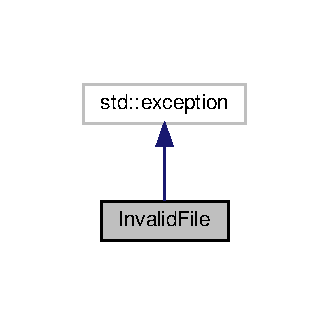
\includegraphics[width=158pt]{class_invalid_file__inherit__graph}
\end{center}
\end{figure}


Collaboration diagram for Invalid\+File\+:
\nopagebreak
\begin{figure}[H]
\begin{center}
\leavevmode
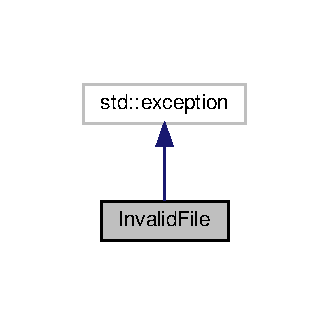
\includegraphics[width=158pt]{class_invalid_file__coll__graph}
\end{center}
\end{figure}
\subsection*{Public Member Functions}
\begin{DoxyCompactItemize}
\item 
\hyperlink{class_invalid_file_ae8e9774922e4413b547b927678450403}{Invalid\+File} (const std\+::string \&message=\char`\"{}\char`\"{})
\item 
const char $\ast$ \hyperlink{class_invalid_file_a1652de4e9e153ed2bf68847b60fa97f4}{what} () const  throw ()
\begin{DoxyCompactList}\small\item\em What to throw upon call. \end{DoxyCompactList}\end{DoxyCompactItemize}


\subsection{Detailed Description}
\hyperlink{class_invalid_file}{Invalid\+File} exception for parsers. 

\subsection{Constructor \& Destructor Documentation}
\mbox{\Hypertarget{class_invalid_file_ae8e9774922e4413b547b927678450403}\label{class_invalid_file_ae8e9774922e4413b547b927678450403}} 
\index{Invalid\+File@{Invalid\+File}!Invalid\+File@{Invalid\+File}}
\index{Invalid\+File@{Invalid\+File}!Invalid\+File@{Invalid\+File}}
\subsubsection{\texorpdfstring{Invalid\+File()}{InvalidFile()}}
{\footnotesize\ttfamily Invalid\+File\+::\+Invalid\+File (\begin{DoxyParamCaption}\item[{const std\+::string \&}]{message = {\ttfamily \char`\"{}\char`\"{}} }\end{DoxyParamCaption})\hspace{0.3cm}{\ttfamily [inline]}, {\ttfamily [explicit]}}



\subsection{Member Function Documentation}
\mbox{\Hypertarget{class_invalid_file_a1652de4e9e153ed2bf68847b60fa97f4}\label{class_invalid_file_a1652de4e9e153ed2bf68847b60fa97f4}} 
\index{Invalid\+File@{Invalid\+File}!what@{what}}
\index{what@{what}!Invalid\+File@{Invalid\+File}}
\subsubsection{\texorpdfstring{what()}{what()}}
{\footnotesize\ttfamily const char$\ast$ Invalid\+File\+::what (\begin{DoxyParamCaption}{ }\end{DoxyParamCaption}) const throw  ) \hspace{0.3cm}{\ttfamily [inline]}}



What to throw upon call. 

\begin{DoxyReturn}{Returns}
const char$\ast$ 
\end{DoxyReturn}


The documentation for this class was generated from the following file\+:\begin{DoxyCompactItemize}
\item 
/media/diane/\+My Passport/\+U\+M\+D Masters/\+Fall 2021/\+E\+N\+P\+M 808\+X/\+Assignments/\+Midterm/\+A\+C\+M\+E\+\_\+perception\+\_\+proposal/include/\hyperlink{utils_8hpp}{utils.\+hpp}\end{DoxyCompactItemize}

\hypertarget{class_label_parser}{}\section{Label\+Parser Class Reference}
\label{class_label_parser}\index{Label\+Parser@{Label\+Parser}}


{\ttfamily \#include $<$Label\+Parser.\+hpp$>$}

\subsection*{Public Member Functions}
\begin{DoxyCompactItemize}
\item 
std\+::shared\+\_\+ptr$<$ \hyperlink{struct_test_image}{Test\+Image} $>$ \hyperlink{class_label_parser_ac524e2136bcf06560e53fadf0c7eb9ad}{parse\+\_\+file} (const std\+::string \&file\+\_\+path)
\begin{DoxyCompactList}\small\item\em Parses labeled image file. \end{DoxyCompactList}\item 
std\+::vector$<$ std\+::shared\+\_\+ptr$<$ \hyperlink{struct_test_image}{Test\+Image} $>$ $>$ \hyperlink{class_label_parser_a2de825ad0f48b9e5b8b3a27c2cf697a7}{read\+\_\+labeled\+\_\+test\+\_\+images} (const std\+::string \&dir\+\_\+path)
\begin{DoxyCompactList}\small\item\em Parses ever labeled image file in the input directory. \end{DoxyCompactList}\end{DoxyCompactItemize}


\subsection{Member Function Documentation}
\mbox{\Hypertarget{class_label_parser_ac524e2136bcf06560e53fadf0c7eb9ad}\label{class_label_parser_ac524e2136bcf06560e53fadf0c7eb9ad}} 
\index{Label\+Parser@{Label\+Parser}!parse\+\_\+file@{parse\+\_\+file}}
\index{parse\+\_\+file@{parse\+\_\+file}!Label\+Parser@{Label\+Parser}}
\subsubsection{\texorpdfstring{parse\+\_\+file()}{parse\_file()}}
{\footnotesize\ttfamily std\+::shared\+\_\+ptr$<$\hyperlink{struct_test_image}{Test\+Image}$>$ Label\+Parser\+::parse\+\_\+file (\begin{DoxyParamCaption}\item[{const std\+::string \&}]{file\+\_\+path }\end{DoxyParamCaption})}



Parses labeled image file. 


\begin{DoxyParams}{Parameters}
{\em file\+\_\+path} & std\+::string \\
\hline
\end{DoxyParams}
\begin{DoxyReturn}{Returns}
std\+::shared\+\_\+ptr$<$\+Test\+Image$>$ shared pointer to a \hyperlink{struct_test_image}{Test\+Image} instance. 
\end{DoxyReturn}
\mbox{\Hypertarget{class_label_parser_a2de825ad0f48b9e5b8b3a27c2cf697a7}\label{class_label_parser_a2de825ad0f48b9e5b8b3a27c2cf697a7}} 
\index{Label\+Parser@{Label\+Parser}!read\+\_\+labeled\+\_\+test\+\_\+images@{read\+\_\+labeled\+\_\+test\+\_\+images}}
\index{read\+\_\+labeled\+\_\+test\+\_\+images@{read\+\_\+labeled\+\_\+test\+\_\+images}!Label\+Parser@{Label\+Parser}}
\subsubsection{\texorpdfstring{read\+\_\+labeled\+\_\+test\+\_\+images()}{read\_labeled\_test\_images()}}
{\footnotesize\ttfamily std\+::vector$<$std\+::shared\+\_\+ptr$<$\hyperlink{struct_test_image}{Test\+Image}$>$ $>$ Label\+Parser\+::read\+\_\+labeled\+\_\+test\+\_\+images (\begin{DoxyParamCaption}\item[{const std\+::string \&}]{dir\+\_\+path }\end{DoxyParamCaption})}



Parses ever labeled image file in the input directory. 


\begin{DoxyParams}{Parameters}
{\em dir\+\_\+path} & path of the desired dir \\
\hline
\end{DoxyParams}
\begin{DoxyReturn}{Returns}
std\+::vector$<$std\+::shared\+\_\+ptr$<$\+Test\+Image$>$ $>$ 
\end{DoxyReturn}


The documentation for this class was generated from the following file\+:\begin{DoxyCompactItemize}
\item 
/media/diane/\+My Passport/\+U\+M\+D Masters/\+Fall 2021/\+E\+N\+P\+M 808\+X/\+Assignments/\+Midterm/\+A\+C\+M\+E\+\_\+perception\+\_\+proposal/include/\hyperlink{_label_parser_8hpp}{Label\+Parser.\+hpp}\end{DoxyCompactItemize}

\hypertarget{class_param_parser}{}\section{Param\+Parser Class Reference}
\label{class_param_parser}\index{Param\+Parser@{Param\+Parser}}


{\ttfamily \#include $<$Param\+Parser.\+hpp$>$}

\subsection*{Public Member Functions}
\begin{DoxyCompactItemize}
\item 
\hyperlink{class_param_parser_a1acf0bbc9dd08f878c050d530e2407ce}{Param\+Parser} (const std\+::vector$<$ \hyperlink{struct_var}{Var} $>$ \&var\+\_\+list)
\item 
std\+::array$<$ std\+::string, 2 $>$ \hyperlink{class_param_parser_a93452e252390edc07934ea08f5dce351}{get\+\_\+unit} (const std\+::string \&line)
\begin{DoxyCompactList}\small\item\em Extracts the unit from a string. \end{DoxyCompactList}\item 
std\+::array$<$ std\+::string, 3 $>$ \hyperlink{class_param_parser_a4a57d55f9ccfa1e728763fd6ddc844f3}{split\+\_\+variable} (const std\+::string \&line)
\begin{DoxyCompactList}\small\item\em Splits variable into name, value, unit. \end{DoxyCompactList}\item 
double \hyperlink{class_param_parser_a2c0289b9e481c8aabd8f68a30d15d906}{set\+\_\+variable} (const std\+::array$<$ std\+::string, 3 $>$ \&var)
\begin{DoxyCompactList}\small\item\em Uses the value and unit to determine true value for a given variable. \end{DoxyCompactList}\item 
std\+::unordered\+\_\+map$<$ std\+::string, double $>$ \hyperlink{class_param_parser_ad55f29f701b36351486e4afb8a70b338}{parse\+\_\+robot\+\_\+params} (std\+::string file)
\begin{DoxyCompactList}\small\item\em Parse robot parameter textfile. \end{DoxyCompactList}\end{DoxyCompactItemize}


\subsection{Constructor \& Destructor Documentation}
\mbox{\Hypertarget{class_param_parser_a1acf0bbc9dd08f878c050d530e2407ce}\label{class_param_parser_a1acf0bbc9dd08f878c050d530e2407ce}} 
\index{Param\+Parser@{Param\+Parser}!Param\+Parser@{Param\+Parser}}
\index{Param\+Parser@{Param\+Parser}!Param\+Parser@{Param\+Parser}}
\subsubsection{\texorpdfstring{Param\+Parser()}{ParamParser()}}
{\footnotesize\ttfamily Param\+Parser\+::\+Param\+Parser (\begin{DoxyParamCaption}\item[{const std\+::vector$<$ \hyperlink{struct_var}{Var} $>$ \&}]{var\+\_\+list }\end{DoxyParamCaption})\hspace{0.3cm}{\ttfamily [inline]}}



\subsection{Member Function Documentation}
\mbox{\Hypertarget{class_param_parser_a93452e252390edc07934ea08f5dce351}\label{class_param_parser_a93452e252390edc07934ea08f5dce351}} 
\index{Param\+Parser@{Param\+Parser}!get\+\_\+unit@{get\+\_\+unit}}
\index{get\+\_\+unit@{get\+\_\+unit}!Param\+Parser@{Param\+Parser}}
\subsubsection{\texorpdfstring{get\+\_\+unit()}{get\_unit()}}
{\footnotesize\ttfamily std\+::array$<$std\+::string, 2$>$ Param\+Parser\+::get\+\_\+unit (\begin{DoxyParamCaption}\item[{const std\+::string \&}]{line }\end{DoxyParamCaption})}



Extracts the unit from a string. 


\begin{DoxyParams}{Parameters}
{\em line} & of text \\
\hline
\end{DoxyParams}
\begin{DoxyReturn}{Returns}
the unit specified and the rest of the text on that line 
\end{DoxyReturn}
\mbox{\Hypertarget{class_param_parser_ad55f29f701b36351486e4afb8a70b338}\label{class_param_parser_ad55f29f701b36351486e4afb8a70b338}} 
\index{Param\+Parser@{Param\+Parser}!parse\+\_\+robot\+\_\+params@{parse\+\_\+robot\+\_\+params}}
\index{parse\+\_\+robot\+\_\+params@{parse\+\_\+robot\+\_\+params}!Param\+Parser@{Param\+Parser}}
\subsubsection{\texorpdfstring{parse\+\_\+robot\+\_\+params()}{parse\_robot\_params()}}
{\footnotesize\ttfamily std\+::unordered\+\_\+map$<$std\+::string, double$>$ Param\+Parser\+::parse\+\_\+robot\+\_\+params (\begin{DoxyParamCaption}\item[{std\+::string}]{file }\end{DoxyParamCaption})}



Parse robot parameter textfile. 


\begin{DoxyParams}{Parameters}
{\em file} & name and path of the robot parameter file \\
\hline
\end{DoxyParams}
\begin{DoxyReturn}{Returns}
a dictionary corresponding to each robot parameter and their corresponding values. 
\end{DoxyReturn}
\mbox{\Hypertarget{class_param_parser_a2c0289b9e481c8aabd8f68a30d15d906}\label{class_param_parser_a2c0289b9e481c8aabd8f68a30d15d906}} 
\index{Param\+Parser@{Param\+Parser}!set\+\_\+variable@{set\+\_\+variable}}
\index{set\+\_\+variable@{set\+\_\+variable}!Param\+Parser@{Param\+Parser}}
\subsubsection{\texorpdfstring{set\+\_\+variable()}{set\_variable()}}
{\footnotesize\ttfamily double Param\+Parser\+::set\+\_\+variable (\begin{DoxyParamCaption}\item[{const std\+::array$<$ std\+::string, 3 $>$ \&}]{var }\end{DoxyParamCaption})}



Uses the value and unit to determine true value for a given variable. 


\begin{DoxyParams}{Parameters}
{\em var} & Variable information \\
\hline
\end{DoxyParams}
\begin{DoxyReturn}{Returns}
true variable value 
\end{DoxyReturn}
\mbox{\Hypertarget{class_param_parser_a4a57d55f9ccfa1e728763fd6ddc844f3}\label{class_param_parser_a4a57d55f9ccfa1e728763fd6ddc844f3}} 
\index{Param\+Parser@{Param\+Parser}!split\+\_\+variable@{split\+\_\+variable}}
\index{split\+\_\+variable@{split\+\_\+variable}!Param\+Parser@{Param\+Parser}}
\subsubsection{\texorpdfstring{split\+\_\+variable()}{split\_variable()}}
{\footnotesize\ttfamily std\+::array$<$std\+::string, 3$>$ Param\+Parser\+::split\+\_\+variable (\begin{DoxyParamCaption}\item[{const std\+::string \&}]{line }\end{DoxyParamCaption})}



Splits variable into name, value, unit. 


\begin{DoxyParams}{Parameters}
{\em line} & of text \\
\hline
\end{DoxyParams}
\begin{DoxyReturn}{Returns}
an array of strings corresponding to name, value, unit 
\end{DoxyReturn}


The documentation for this class was generated from the following file\+:\begin{DoxyCompactItemize}
\item 
/media/diane/\+My Passport/\+U\+M\+D Masters/\+Fall 2021/\+E\+N\+P\+M 808\+X/\+Assignments/\+Midterm/\+A\+C\+M\+E\+\_\+perception\+\_\+proposal/include/\hyperlink{_param_parser_8hpp}{Param\+Parser.\+hpp}\end{DoxyCompactItemize}

\hypertarget{class_position_estimator}{}\section{Position\+Estimator Class Reference}
\label{class_position_estimator}\index{Position\+Estimator@{Position\+Estimator}}


{\ttfamily \#include $<$Position\+Estimator.\+hpp$>$}

\subsection*{Public Member Functions}
\begin{DoxyCompactItemize}
\item 
\hyperlink{class_position_estimator_a39de44247f8c8feaed5bd1de8438245f}{Position\+Estimator} (double x, double y, double z, double pitch, double f\+\_\+x, double f\+\_\+y, double s, double px, double py, double avg\+\_\+height)
\item 
\hyperlink{class_position_estimator_af0b8305de010b7f15f0b18499d8d50c3}{Position\+Estimator} (const std\+::unordered\+\_\+map$<$ std\+::string, double $>$ \&robot\+\_\+params)
\item 
bool \hyperlink{class_position_estimator_a6414758ee472d223f6b97369abe27968}{threshold\+\_\+frame} (double probability)
\begin{DoxyCompactList}\small\item\em This function removes noise by discarding frames with low probability of human detection. \end{DoxyCompactList}\item 
double \hyperlink{class_position_estimator_aaa7e82a010bfb5dbcc795af9718c9eb0}{approximate\+\_\+camera\+\_\+z} (\hyperlink{struct_detection}{Detection} \&detection)
\begin{DoxyCompactList}\small\item\em This function approximates the z location of the human in the C\+A\+M\+E\+RA frame based on the size of the bounding box. \end{DoxyCompactList}\item 
std\+::array$<$ double, 3 $>$ \hyperlink{class_position_estimator_a90f4ced196e47ac347fcf53e834fbcab}{estimate\+\_\+xyz} (\hyperlink{struct_detection}{Detection} \&)
\begin{DoxyCompactList}\small\item\em This method estimates the xyz position of a S\+I\+N\+G\+LE detected human in the W\+O\+R\+LD frame. \end{DoxyCompactList}\item 
std\+::vector$<$ std\+::array$<$ double, 3 $>$ $>$ \hyperlink{class_position_estimator_a9bc700bc3de4749f5ec40a892c52a09d}{estimate\+\_\+all\+\_\+xyz} (std\+::vector$<$ \hyperlink{struct_detection}{Detection} $>$ \&detection)
\begin{DoxyCompactList}\small\item\em This method estimates the xyz position of E\+A\+CH detected human in the W\+O\+R\+LD frame. \end{DoxyCompactList}\item 
const Eigen\+::\+Matrix$<$ double, 4, 4 $>$ \& \hyperlink{class_position_estimator_a12ae9fe6ea2f7ca1e2054e018c5dabf5}{get\+\_\+cam2robot\+\_\+transform} ()
\begin{DoxyCompactList}\small\item\em Get the cam2robot transform object. \end{DoxyCompactList}\item 
const Eigen\+::\+Matrix$<$ double, 3, 3 $>$ \& \hyperlink{class_position_estimator_a6832a1905352d24cbc834f2f205ba09b}{get\+\_\+inv\+\_\+camera\+\_\+matrix} ()
\begin{DoxyCompactList}\small\item\em Get the camera matrix object. \end{DoxyCompactList}\end{DoxyCompactItemize}


\subsection{Constructor \& Destructor Documentation}
\mbox{\Hypertarget{class_position_estimator_a39de44247f8c8feaed5bd1de8438245f}\label{class_position_estimator_a39de44247f8c8feaed5bd1de8438245f}} 
\index{Position\+Estimator@{Position\+Estimator}!Position\+Estimator@{Position\+Estimator}}
\index{Position\+Estimator@{Position\+Estimator}!Position\+Estimator@{Position\+Estimator}}
\subsubsection{\texorpdfstring{Position\+Estimator()}{PositionEstimator()}\hspace{0.1cm}{\footnotesize\ttfamily [1/2]}}
{\footnotesize\ttfamily Position\+Estimator\+::\+Position\+Estimator (\begin{DoxyParamCaption}\item[{double}]{x,  }\item[{double}]{y,  }\item[{double}]{z,  }\item[{double}]{pitch,  }\item[{double}]{f\+\_\+x,  }\item[{double}]{f\+\_\+y,  }\item[{double}]{s,  }\item[{double}]{px,  }\item[{double}]{py,  }\item[{double}]{avg\+\_\+height }\end{DoxyParamCaption})\hspace{0.3cm}{\ttfamily [inline]}}

\mbox{\Hypertarget{class_position_estimator_af0b8305de010b7f15f0b18499d8d50c3}\label{class_position_estimator_af0b8305de010b7f15f0b18499d8d50c3}} 
\index{Position\+Estimator@{Position\+Estimator}!Position\+Estimator@{Position\+Estimator}}
\index{Position\+Estimator@{Position\+Estimator}!Position\+Estimator@{Position\+Estimator}}
\subsubsection{\texorpdfstring{Position\+Estimator()}{PositionEstimator()}\hspace{0.1cm}{\footnotesize\ttfamily [2/2]}}
{\footnotesize\ttfamily Position\+Estimator\+::\+Position\+Estimator (\begin{DoxyParamCaption}\item[{const std\+::unordered\+\_\+map$<$ std\+::string, double $>$ \&}]{robot\+\_\+params }\end{DoxyParamCaption})\hspace{0.3cm}{\ttfamily [inline]}}



\subsection{Member Function Documentation}
\mbox{\Hypertarget{class_position_estimator_aaa7e82a010bfb5dbcc795af9718c9eb0}\label{class_position_estimator_aaa7e82a010bfb5dbcc795af9718c9eb0}} 
\index{Position\+Estimator@{Position\+Estimator}!approximate\+\_\+camera\+\_\+z@{approximate\+\_\+camera\+\_\+z}}
\index{approximate\+\_\+camera\+\_\+z@{approximate\+\_\+camera\+\_\+z}!Position\+Estimator@{Position\+Estimator}}
\subsubsection{\texorpdfstring{approximate\+\_\+camera\+\_\+z()}{approximate\_camera\_z()}}
{\footnotesize\ttfamily double Position\+Estimator\+::approximate\+\_\+camera\+\_\+z (\begin{DoxyParamCaption}\item[{\hyperlink{struct_detection}{Detection} \&}]{detection }\end{DoxyParamCaption})}



This function approximates the z location of the human in the C\+A\+M\+E\+RA frame based on the size of the bounding box. 


\begin{DoxyParams}{Parameters}
{\em detection} & \hyperlink{struct_detection}{Detection} obj \\
\hline
\end{DoxyParams}
\begin{DoxyReturn}{Returns}
approximate depth of human in camera frame U\+N\+IT\+: \mbox{[}m\mbox{]} 
\end{DoxyReturn}
\mbox{\Hypertarget{class_position_estimator_a9bc700bc3de4749f5ec40a892c52a09d}\label{class_position_estimator_a9bc700bc3de4749f5ec40a892c52a09d}} 
\index{Position\+Estimator@{Position\+Estimator}!estimate\+\_\+all\+\_\+xyz@{estimate\+\_\+all\+\_\+xyz}}
\index{estimate\+\_\+all\+\_\+xyz@{estimate\+\_\+all\+\_\+xyz}!Position\+Estimator@{Position\+Estimator}}
\subsubsection{\texorpdfstring{estimate\+\_\+all\+\_\+xyz()}{estimate\_all\_xyz()}}
{\footnotesize\ttfamily std\+::vector$<$std\+::array$<$double, 3$>$ $>$ Position\+Estimator\+::estimate\+\_\+all\+\_\+xyz (\begin{DoxyParamCaption}\item[{std\+::vector$<$ \hyperlink{struct_detection}{Detection} $>$ \&}]{detection }\end{DoxyParamCaption})}



This method estimates the xyz position of E\+A\+CH detected human in the W\+O\+R\+LD frame. 


\begin{DoxyParams}{Parameters}
{\em detections} & vector of \hyperlink{struct_detection}{Detection} objs \\
\hline
\end{DoxyParams}
\begin{DoxyReturn}{Returns}
std\+::vector$<$std\+::array$<$double, 3$>$$>$\+: x, y, z position of E\+A\+CH human in R\+O\+B\+OT frame U\+N\+IT\+: \mbox{[}m\mbox{]} 
\end{DoxyReturn}
\mbox{\Hypertarget{class_position_estimator_a90f4ced196e47ac347fcf53e834fbcab}\label{class_position_estimator_a90f4ced196e47ac347fcf53e834fbcab}} 
\index{Position\+Estimator@{Position\+Estimator}!estimate\+\_\+xyz@{estimate\+\_\+xyz}}
\index{estimate\+\_\+xyz@{estimate\+\_\+xyz}!Position\+Estimator@{Position\+Estimator}}
\subsubsection{\texorpdfstring{estimate\+\_\+xyz()}{estimate\_xyz()}}
{\footnotesize\ttfamily std\+::array$<$double, 3$>$ Position\+Estimator\+::estimate\+\_\+xyz (\begin{DoxyParamCaption}\item[{\hyperlink{struct_detection}{Detection} \&}]{ }\end{DoxyParamCaption})}



This method estimates the xyz position of a S\+I\+N\+G\+LE detected human in the W\+O\+R\+LD frame. 


\begin{DoxyParams}{Parameters}
{\em detection} & \hyperlink{struct_detection}{Detection} obj \\
\hline
\end{DoxyParams}
\begin{DoxyReturn}{Returns}
std\+::array$<$double, 3$>$\+: x, y, z position of a single human. 
\end{DoxyReturn}
\mbox{\Hypertarget{class_position_estimator_a12ae9fe6ea2f7ca1e2054e018c5dabf5}\label{class_position_estimator_a12ae9fe6ea2f7ca1e2054e018c5dabf5}} 
\index{Position\+Estimator@{Position\+Estimator}!get\+\_\+cam2robot\+\_\+transform@{get\+\_\+cam2robot\+\_\+transform}}
\index{get\+\_\+cam2robot\+\_\+transform@{get\+\_\+cam2robot\+\_\+transform}!Position\+Estimator@{Position\+Estimator}}
\subsubsection{\texorpdfstring{get\+\_\+cam2robot\+\_\+transform()}{get\_cam2robot\_transform()}}
{\footnotesize\ttfamily const Eigen\+::\+Matrix$<$double, 4, 4$>$\& Position\+Estimator\+::get\+\_\+cam2robot\+\_\+transform (\begin{DoxyParamCaption}{ }\end{DoxyParamCaption})\hspace{0.3cm}{\ttfamily [inline]}}



Get the cam2robot transform object. 

\begin{DoxyReturn}{Returns}
const Eigen\+::\+Matrix$<$double, 4, 4$>$\& 
\end{DoxyReturn}
\mbox{\Hypertarget{class_position_estimator_a6832a1905352d24cbc834f2f205ba09b}\label{class_position_estimator_a6832a1905352d24cbc834f2f205ba09b}} 
\index{Position\+Estimator@{Position\+Estimator}!get\+\_\+inv\+\_\+camera\+\_\+matrix@{get\+\_\+inv\+\_\+camera\+\_\+matrix}}
\index{get\+\_\+inv\+\_\+camera\+\_\+matrix@{get\+\_\+inv\+\_\+camera\+\_\+matrix}!Position\+Estimator@{Position\+Estimator}}
\subsubsection{\texorpdfstring{get\+\_\+inv\+\_\+camera\+\_\+matrix()}{get\_inv\_camera\_matrix()}}
{\footnotesize\ttfamily const Eigen\+::\+Matrix$<$double, 3, 3$>$\& Position\+Estimator\+::get\+\_\+inv\+\_\+camera\+\_\+matrix (\begin{DoxyParamCaption}{ }\end{DoxyParamCaption})\hspace{0.3cm}{\ttfamily [inline]}}



Get the camera matrix object. 

\begin{DoxyReturn}{Returns}
const Eigen\+::\+Matrix$<$2, 2, double$>$\& 
\end{DoxyReturn}
\mbox{\Hypertarget{class_position_estimator_a6414758ee472d223f6b97369abe27968}\label{class_position_estimator_a6414758ee472d223f6b97369abe27968}} 
\index{Position\+Estimator@{Position\+Estimator}!threshold\+\_\+frame@{threshold\+\_\+frame}}
\index{threshold\+\_\+frame@{threshold\+\_\+frame}!Position\+Estimator@{Position\+Estimator}}
\subsubsection{\texorpdfstring{threshold\+\_\+frame()}{threshold\_frame()}}
{\footnotesize\ttfamily bool Position\+Estimator\+::threshold\+\_\+frame (\begin{DoxyParamCaption}\item[{double}]{probability }\end{DoxyParamCaption})}



This function removes noise by discarding frames with low probability of human detection. 


\begin{DoxyParams}{Parameters}
{\em probability} & Human detection probability \\
\hline
\end{DoxyParams}
\begin{DoxyReturn}{Returns}
whether we have decided the frame has a human in it or not 
\end{DoxyReturn}


The documentation for this class was generated from the following file\+:\begin{DoxyCompactItemize}
\item 
/media/diane/\+My Passport/\+U\+M\+D Masters/\+Fall 2021/\+E\+N\+P\+M 808\+X/\+Assignments/\+Midterm/\+A\+C\+M\+E\+\_\+perception\+\_\+proposal/include/\hyperlink{_position_estimator_8hpp}{Position\+Estimator.\+hpp}\end{DoxyCompactItemize}

\hypertarget{struct_test_image}{}\section{Test\+Image Struct Reference}
\label{struct_test_image}\index{Test\+Image@{Test\+Image}}


{\ttfamily \#include $<$Label\+Parser.\+hpp$>$}

\subsection*{Public Attributes}
\begin{DoxyCompactItemize}
\item 
std\+::string \hyperlink{struct_test_image_a53e7396d578566495ce7a5291b5e8dc5}{name}
\item 
std\+::vector$<$ \hyperlink{struct_detection}{Detection} $>$ \hyperlink{struct_test_image_ae2a58c7febd059cc3b2cc4c74bf81ba5}{all\+\_\+detections} \{\}
\item 
cv\+::\+Mat \hyperlink{struct_test_image_a021bb1d1bd261d9237e5c4298ade0fc4}{img}
\end{DoxyCompactItemize}


\subsection{Member Data Documentation}
\mbox{\Hypertarget{struct_test_image_ae2a58c7febd059cc3b2cc4c74bf81ba5}\label{struct_test_image_ae2a58c7febd059cc3b2cc4c74bf81ba5}} 
\index{Test\+Image@{Test\+Image}!all\+\_\+detections@{all\+\_\+detections}}
\index{all\+\_\+detections@{all\+\_\+detections}!Test\+Image@{Test\+Image}}
\subsubsection{\texorpdfstring{all\+\_\+detections}{all\_detections}}
{\footnotesize\ttfamily std\+::vector$<$\hyperlink{struct_detection}{Detection}$>$ Test\+Image\+::all\+\_\+detections \{\}}

\mbox{\Hypertarget{struct_test_image_a021bb1d1bd261d9237e5c4298ade0fc4}\label{struct_test_image_a021bb1d1bd261d9237e5c4298ade0fc4}} 
\index{Test\+Image@{Test\+Image}!img@{img}}
\index{img@{img}!Test\+Image@{Test\+Image}}
\subsubsection{\texorpdfstring{img}{img}}
{\footnotesize\ttfamily cv\+::\+Mat Test\+Image\+::img}

\mbox{\Hypertarget{struct_test_image_a53e7396d578566495ce7a5291b5e8dc5}\label{struct_test_image_a53e7396d578566495ce7a5291b5e8dc5}} 
\index{Test\+Image@{Test\+Image}!name@{name}}
\index{name@{name}!Test\+Image@{Test\+Image}}
\subsubsection{\texorpdfstring{name}{name}}
{\footnotesize\ttfamily std\+::string Test\+Image\+::name}



The documentation for this struct was generated from the following file\+:\begin{DoxyCompactItemize}
\item 
/media/diane/\+My Passport/\+U\+M\+D Masters/\+Fall 2021/\+E\+N\+P\+M 808\+X/\+Assignments/\+Midterm/\+A\+C\+M\+E\+\_\+perception\+\_\+proposal/include/\hyperlink{_label_parser_8hpp}{Label\+Parser.\+hpp}\end{DoxyCompactItemize}

\hypertarget{struct_var}{}\section{Var Struct Reference}
\label{struct_var}\index{Var@{Var}}


{\ttfamily \#include $<$Param\+Parser.\+hpp$>$}

\subsection*{Public Member Functions}
\begin{DoxyCompactItemize}
\item 
\hyperlink{struct_var_acd32463974964de2ddbb3de36a508ed0}{Var} (std\+::string \+\_\+name, std\+::string \+\_\+default\+\_\+unit)
\end{DoxyCompactItemize}
\subsection*{Public Attributes}
\begin{DoxyCompactItemize}
\item 
std\+::string \hyperlink{struct_var_ad112053ba9381eb7b8b26b3c5702410a}{name}
\item 
std\+::string \hyperlink{struct_var_adadd3377feb65e8bc4cfa10978918b4d}{default\+\_\+unit}
\end{DoxyCompactItemize}


\subsection{Constructor \& Destructor Documentation}
\mbox{\Hypertarget{struct_var_acd32463974964de2ddbb3de36a508ed0}\label{struct_var_acd32463974964de2ddbb3de36a508ed0}} 
\index{Var@{Var}!Var@{Var}}
\index{Var@{Var}!Var@{Var}}
\subsubsection{\texorpdfstring{Var()}{Var()}}
{\footnotesize\ttfamily Var\+::\+Var (\begin{DoxyParamCaption}\item[{std\+::string}]{\+\_\+name,  }\item[{std\+::string}]{\+\_\+default\+\_\+unit }\end{DoxyParamCaption})\hspace{0.3cm}{\ttfamily [inline]}}



\subsection{Member Data Documentation}
\mbox{\Hypertarget{struct_var_adadd3377feb65e8bc4cfa10978918b4d}\label{struct_var_adadd3377feb65e8bc4cfa10978918b4d}} 
\index{Var@{Var}!default\+\_\+unit@{default\+\_\+unit}}
\index{default\+\_\+unit@{default\+\_\+unit}!Var@{Var}}
\subsubsection{\texorpdfstring{default\+\_\+unit}{default\_unit}}
{\footnotesize\ttfamily std\+::string Var\+::default\+\_\+unit}

\mbox{\Hypertarget{struct_var_ad112053ba9381eb7b8b26b3c5702410a}\label{struct_var_ad112053ba9381eb7b8b26b3c5702410a}} 
\index{Var@{Var}!name@{name}}
\index{name@{name}!Var@{Var}}
\subsubsection{\texorpdfstring{name}{name}}
{\footnotesize\ttfamily std\+::string Var\+::name}



The documentation for this struct was generated from the following file\+:\begin{DoxyCompactItemize}
\item 
/media/diane/\+My Passport/\+U\+M\+D Masters/\+Fall 2021/\+E\+N\+P\+M 808\+X/\+Assignments/\+Midterm/\+A\+C\+M\+E\+\_\+perception\+\_\+proposal/include/\hyperlink{_param_parser_8hpp}{Param\+Parser.\+hpp}\end{DoxyCompactItemize}

\hypertarget{class_vision_a_p_i}{}\section{Vision\+A\+PI Class Reference}
\label{class_vision_a_p_i}\index{Vision\+A\+PI@{Vision\+A\+PI}}


{\ttfamily \#include $<$Vision\+A\+P\+I.\+hpp$>$}

\subsection*{Public Member Functions}
\begin{DoxyCompactItemize}
\item 
\hyperlink{class_vision_a_p_i_a1ebc6d928618773c2fa97e2e593afaa4}{Vision\+A\+PI} (const std\+::unordered\+\_\+map$<$ std\+::string, double $>$ \&\+\_\+robot\+\_\+params)
\item 
std\+::vector$<$ std\+::array$<$ double, 3 $>$ $>$ \hyperlink{class_vision_a_p_i_a2abdb5d06b3c66789a970d541a44f55e}{get\+\_\+xyz} (cv\+::\+Mat)
\begin{DoxyCompactList}\small\item\em This method takes an image, finds all people within the image, and outputs the estimated postions in the R\+O\+B\+OT frame. \end{DoxyCompactList}\end{DoxyCompactItemize}


\subsection{Constructor \& Destructor Documentation}
\mbox{\Hypertarget{class_vision_a_p_i_a1ebc6d928618773c2fa97e2e593afaa4}\label{class_vision_a_p_i_a1ebc6d928618773c2fa97e2e593afaa4}} 
\index{Vision\+A\+PI@{Vision\+A\+PI}!Vision\+A\+PI@{Vision\+A\+PI}}
\index{Vision\+A\+PI@{Vision\+A\+PI}!Vision\+A\+PI@{Vision\+A\+PI}}
\subsubsection{\texorpdfstring{Vision\+A\+P\+I()}{VisionAPI()}}
{\footnotesize\ttfamily Vision\+A\+P\+I\+::\+Vision\+A\+PI (\begin{DoxyParamCaption}\item[{const std\+::unordered\+\_\+map$<$ std\+::string, double $>$ \&}]{\+\_\+robot\+\_\+params }\end{DoxyParamCaption})\hspace{0.3cm}{\ttfamily [inline]}}



\subsection{Member Function Documentation}
\mbox{\Hypertarget{class_vision_a_p_i_a2abdb5d06b3c66789a970d541a44f55e}\label{class_vision_a_p_i_a2abdb5d06b3c66789a970d541a44f55e}} 
\index{Vision\+A\+PI@{Vision\+A\+PI}!get\+\_\+xyz@{get\+\_\+xyz}}
\index{get\+\_\+xyz@{get\+\_\+xyz}!Vision\+A\+PI@{Vision\+A\+PI}}
\subsubsection{\texorpdfstring{get\+\_\+xyz()}{get\_xyz()}}
{\footnotesize\ttfamily std\+::vector$<$std\+::array$<$double, 3$>$ $>$ Vision\+A\+P\+I\+::get\+\_\+xyz (\begin{DoxyParamCaption}\item[{cv\+::\+Mat}]{ }\end{DoxyParamCaption})}



This method takes an image, finds all people within the image, and outputs the estimated postions in the R\+O\+B\+OT frame. 


\begin{DoxyParams}{Parameters}
{\em img} & \\
\hline
\end{DoxyParams}
\begin{DoxyReturn}{Returns}
All estimated x, y, z positions of people in a given image. 
\end{DoxyReturn}


The documentation for this class was generated from the following file\+:\begin{DoxyCompactItemize}
\item 
/media/diane/\+My Passport/\+U\+M\+D Masters/\+Fall 2021/\+E\+N\+P\+M 808\+X/\+Assignments/\+Midterm/\+A\+C\+M\+E\+\_\+perception\+\_\+proposal/include/\hyperlink{_vision_a_p_i_8hpp}{Vision\+A\+P\+I.\+hpp}\end{DoxyCompactItemize}

\chapter{File Documentation}
\hypertarget{_detection_8hpp}{}\section{/media/diane/\+My Passport/\+U\+MD Masters/\+Fall 2021/\+E\+N\+PM 808\+X/\+Assignments/\+Midterm/\+A\+C\+M\+E\+\_\+perception\+\_\+proposal/include/\+Detection.hpp File Reference}
\label{_detection_8hpp}\index{/media/diane/\+My Passport/\+U\+M\+D Masters/\+Fall 2021/\+E\+N\+P\+M 808\+X/\+Assignments/\+Midterm/\+A\+C\+M\+E\+\_\+perception\+\_\+proposal/include/\+Detection.\+hpp@{/media/diane/\+My Passport/\+U\+M\+D Masters/\+Fall 2021/\+E\+N\+P\+M 808\+X/\+Assignments/\+Midterm/\+A\+C\+M\+E\+\_\+perception\+\_\+proposal/include/\+Detection.\+hpp}}
This graph shows which files directly or indirectly include this file\+:
\nopagebreak
\begin{figure}[H]
\begin{center}
\leavevmode
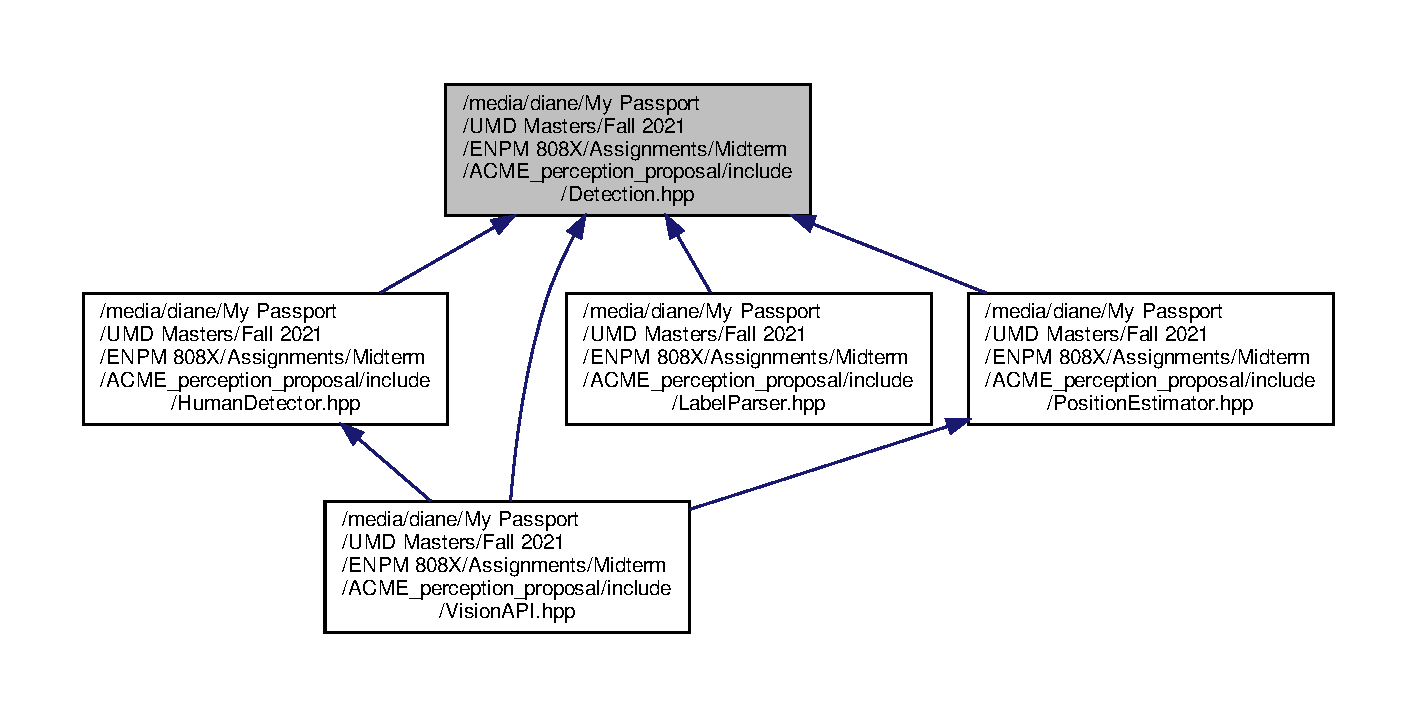
\includegraphics[width=350pt]{_detection_8hpp__dep__incl}
\end{center}
\end{figure}
\subsection*{Classes}
\begin{DoxyCompactItemize}
\item 
struct \hyperlink{struct_detection}{Detection}
\begin{DoxyCompactList}\small\item\em This struct will be used to pass detection information between the human detector and position estimator classes. See the U\+ML for more information. \end{DoxyCompactList}\end{DoxyCompactItemize}

\hypertarget{_human_detector_8hpp}{}\section{/media/diane/\+My Passport/\+U\+MD Masters/\+Fall 2021/\+E\+N\+PM 808\+X/\+Assignments/\+Midterm/\+A\+C\+M\+E\+\_\+perception\+\_\+proposal/include/\+Human\+Detector.hpp File Reference}
\label{_human_detector_8hpp}\index{/media/diane/\+My Passport/\+U\+M\+D Masters/\+Fall 2021/\+E\+N\+P\+M 808\+X/\+Assignments/\+Midterm/\+A\+C\+M\+E\+\_\+perception\+\_\+proposal/include/\+Human\+Detector.\+hpp@{/media/diane/\+My Passport/\+U\+M\+D Masters/\+Fall 2021/\+E\+N\+P\+M 808\+X/\+Assignments/\+Midterm/\+A\+C\+M\+E\+\_\+perception\+\_\+proposal/include/\+Human\+Detector.\+hpp}}
{\ttfamily \#include $<$array$>$}\newline
{\ttfamily \#include $<$vector$>$}\newline
{\ttfamily \#include $<$string$>$}\newline
{\ttfamily \#include $<$memory$>$}\newline
{\ttfamily \#include $<$unordered\+\_\+map$>$}\newline
{\ttfamily \#include $<$opencv2/opencv.\+hpp$>$}\newline
{\ttfamily \#include \char`\"{}Detection.\+hpp\char`\"{}}\newline
Include dependency graph for Human\+Detector.\+hpp\+:
\nopagebreak
\begin{figure}[H]
\begin{center}
\leavevmode
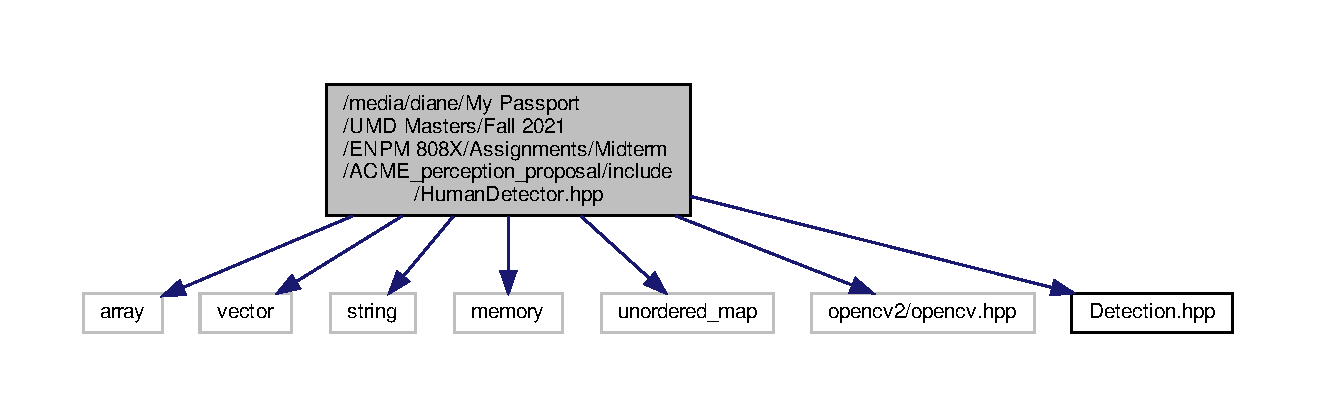
\includegraphics[width=350pt]{_human_detector_8hpp__incl}
\end{center}
\end{figure}
This graph shows which files directly or indirectly include this file\+:
\nopagebreak
\begin{figure}[H]
\begin{center}
\leavevmode
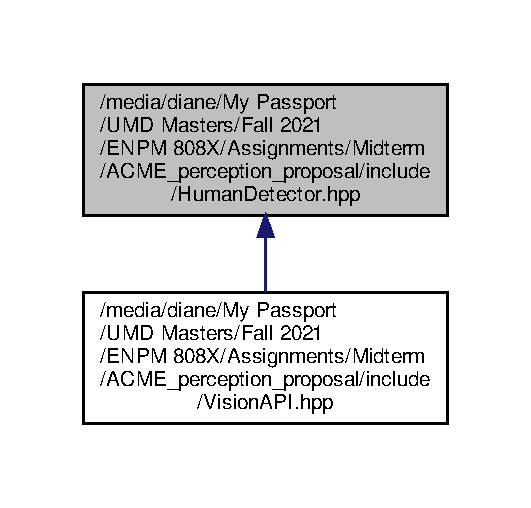
\includegraphics[width=255pt]{_human_detector_8hpp__dep__incl}
\end{center}
\end{figure}
\subsection*{Classes}
\begin{DoxyCompactItemize}
\item 
class \hyperlink{class_human_detector}{Human\+Detector}
\end{DoxyCompactItemize}

\hypertarget{_label_parser_8hpp}{}\section{/media/diane/\+My Passport/\+U\+MD Masters/\+Fall 2021/\+E\+N\+PM 808\+X/\+Assignments/\+Midterm/\+A\+C\+M\+E\+\_\+perception\+\_\+proposal/include/\+Label\+Parser.hpp File Reference}
\label{_label_parser_8hpp}\index{/media/diane/\+My Passport/\+U\+M\+D Masters/\+Fall 2021/\+E\+N\+P\+M 808\+X/\+Assignments/\+Midterm/\+A\+C\+M\+E\+\_\+perception\+\_\+proposal/include/\+Label\+Parser.\+hpp@{/media/diane/\+My Passport/\+U\+M\+D Masters/\+Fall 2021/\+E\+N\+P\+M 808\+X/\+Assignments/\+Midterm/\+A\+C\+M\+E\+\_\+perception\+\_\+proposal/include/\+Label\+Parser.\+hpp}}


Label Parser header.  


{\ttfamily \#include $<$array$>$}\newline
{\ttfamily \#include $<$vector$>$}\newline
{\ttfamily \#include $<$string$>$}\newline
{\ttfamily \#include $<$memory$>$}\newline
{\ttfamily \#include $<$opencv2/opencv.\+hpp$>$}\newline
{\ttfamily \#include \char`\"{}./\+Detection.\+hpp\char`\"{}}\newline
Include dependency graph for Label\+Parser.\+hpp\+:
\nopagebreak
\begin{figure}[H]
\begin{center}
\leavevmode
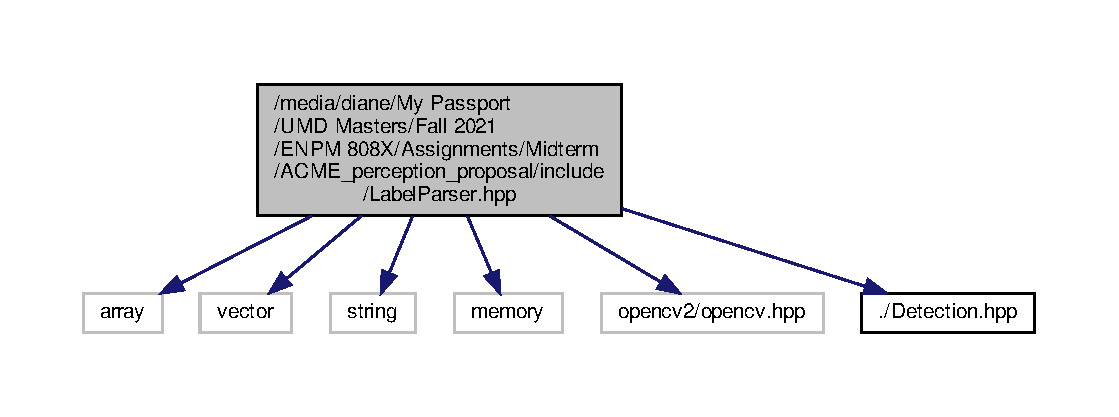
\includegraphics[width=350pt]{_label_parser_8hpp__incl}
\end{center}
\end{figure}
\subsection*{Classes}
\begin{DoxyCompactItemize}
\item 
struct \hyperlink{struct_test_image}{Test\+Image}
\item 
class \hyperlink{class_label_parser}{Label\+Parser}
\end{DoxyCompactItemize}


\subsection{Detailed Description}
Label Parser header. 

\begin{DoxyAuthor}{Author}
Dani Lerner 

Diane Ngo 
\end{DoxyAuthor}
\begin{DoxyVersion}{Version}
0.\+1 
\end{DoxyVersion}
\begin{DoxyDate}{Date}
2021-\/10-\/25
\end{DoxyDate}
\begin{DoxyCopyright}{Copyright}
Copyright (c) 2021 
\end{DoxyCopyright}

\hypertarget{_param_parser_8hpp}{}\section{/media/diane/\+My Passport/\+U\+MD Masters/\+Fall 2021/\+E\+N\+PM 808\+X/\+Assignments/\+Midterm/\+A\+C\+M\+E\+\_\+perception\+\_\+proposal/include/\+Param\+Parser.hpp File Reference}
\label{_param_parser_8hpp}\index{/media/diane/\+My Passport/\+U\+M\+D Masters/\+Fall 2021/\+E\+N\+P\+M 808\+X/\+Assignments/\+Midterm/\+A\+C\+M\+E\+\_\+perception\+\_\+proposal/include/\+Param\+Parser.\+hpp@{/media/diane/\+My Passport/\+U\+M\+D Masters/\+Fall 2021/\+E\+N\+P\+M 808\+X/\+Assignments/\+Midterm/\+A\+C\+M\+E\+\_\+perception\+\_\+proposal/include/\+Param\+Parser.\+hpp}}


Param Parser header.  


{\ttfamily \#include $<$array$>$}\newline
{\ttfamily \#include $<$vector$>$}\newline
{\ttfamily \#include $<$string$>$}\newline
{\ttfamily \#include $<$unordered\+\_\+map$>$}\newline
Include dependency graph for Param\+Parser.\+hpp\+:\nopagebreak
\begin{figure}[H]
\begin{center}
\leavevmode
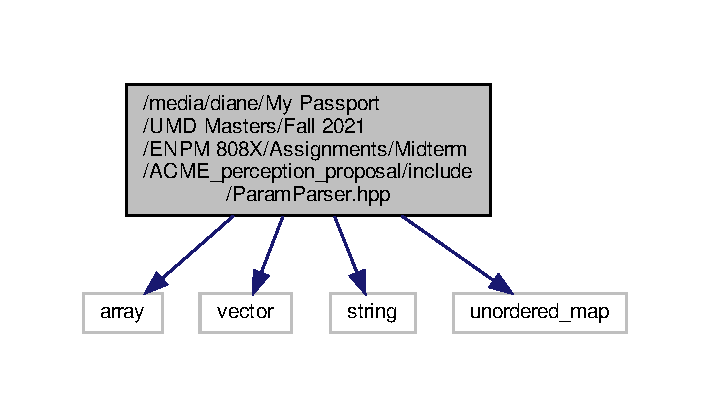
\includegraphics[width=341pt]{_param_parser_8hpp__incl}
\end{center}
\end{figure}
This graph shows which files directly or indirectly include this file\+:
\nopagebreak
\begin{figure}[H]
\begin{center}
\leavevmode
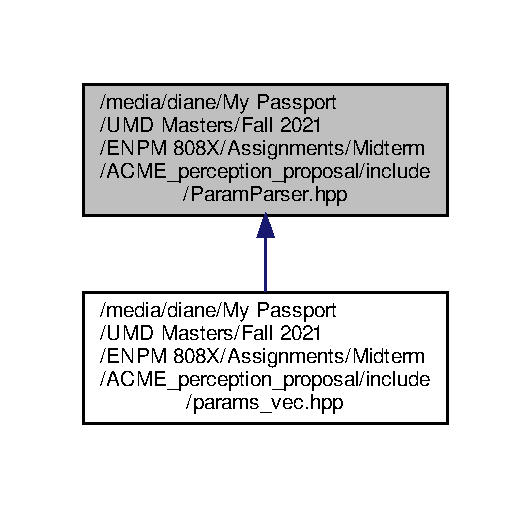
\includegraphics[width=255pt]{_param_parser_8hpp__dep__incl}
\end{center}
\end{figure}
\subsection*{Classes}
\begin{DoxyCompactItemize}
\item 
struct \hyperlink{struct_var}{Var}
\item 
class \hyperlink{class_param_parser}{Param\+Parser}
\end{DoxyCompactItemize}


\subsection{Detailed Description}
Param Parser header. 

\begin{DoxyAuthor}{Author}
Dani Lerner 

Diane Ngo 
\end{DoxyAuthor}
\begin{DoxyVersion}{Version}
0.\+1 
\end{DoxyVersion}
\begin{DoxyDate}{Date}
2021-\/10-\/25
\end{DoxyDate}
\begin{DoxyCopyright}{Copyright}
Copyright (c) 2021 
\end{DoxyCopyright}

\hypertarget{params__vec_8hpp}{}\section{/media/diane/\+My Passport/\+U\+MD Masters/\+Fall 2021/\+E\+N\+PM 808\+X/\+Assignments/\+Midterm/\+A\+C\+M\+E\+\_\+perception\+\_\+proposal/include/params\+\_\+vec.hpp File Reference}
\label{params__vec_8hpp}\index{/media/diane/\+My Passport/\+U\+M\+D Masters/\+Fall 2021/\+E\+N\+P\+M 808\+X/\+Assignments/\+Midterm/\+A\+C\+M\+E\+\_\+perception\+\_\+proposal/include/params\+\_\+vec.\+hpp@{/media/diane/\+My Passport/\+U\+M\+D Masters/\+Fall 2021/\+E\+N\+P\+M 808\+X/\+Assignments/\+Midterm/\+A\+C\+M\+E\+\_\+perception\+\_\+proposal/include/params\+\_\+vec.\+hpp}}


params vector header  


{\ttfamily \#include $<$vector$>$}\newline
{\ttfamily \#include \char`\"{}../include/\+Param\+Parser.\+hpp\char`\"{}}\newline
Include dependency graph for params\+\_\+vec.\+hpp\+:
\nopagebreak
\begin{figure}[H]
\begin{center}
\leavevmode
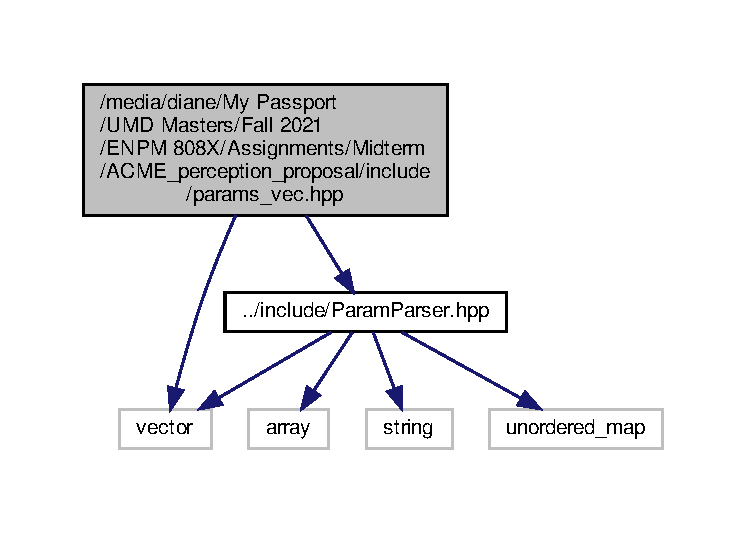
\includegraphics[width=350pt]{params__vec_8hpp__incl}
\end{center}
\end{figure}
\subsection*{Namespaces}
\begin{DoxyCompactItemize}
\item 
 \hyperlink{namespaceall__params}{all\+\_\+params}
\end{DoxyCompactItemize}
\subsection*{Variables}
\begin{DoxyCompactItemize}
\item 
std\+::vector$<$ \hyperlink{struct_var}{Var} $>$ \hyperlink{namespaceall__params_a925d27c82562242237a980dc8c86bc4a}{all\+\_\+params\+::params}
\end{DoxyCompactItemize}


\subsection{Detailed Description}
params vector header 

\begin{DoxyAuthor}{Author}
Dani Lerner 

Diane Ngo 
\end{DoxyAuthor}
\begin{DoxyVersion}{Version}
0.\+1 
\end{DoxyVersion}
\begin{DoxyDate}{Date}
2021-\/10-\/25
\end{DoxyDate}
\begin{DoxyCopyright}{Copyright}
Copyright (c) 2021 
\end{DoxyCopyright}

\hypertarget{_position_estimator_8hpp}{}\section{/media/diane/\+My Passport/\+U\+MD Masters/\+Fall 2021/\+E\+N\+PM 808\+X/\+Assignments/\+Midterm/\+A\+C\+M\+E\+\_\+perception\+\_\+proposal/include/\+Position\+Estimator.hpp File Reference}
\label{_position_estimator_8hpp}\index{/media/diane/\+My Passport/\+U\+M\+D Masters/\+Fall 2021/\+E\+N\+P\+M 808\+X/\+Assignments/\+Midterm/\+A\+C\+M\+E\+\_\+perception\+\_\+proposal/include/\+Position\+Estimator.\+hpp@{/media/diane/\+My Passport/\+U\+M\+D Masters/\+Fall 2021/\+E\+N\+P\+M 808\+X/\+Assignments/\+Midterm/\+A\+C\+M\+E\+\_\+perception\+\_\+proposal/include/\+Position\+Estimator.\+hpp}}
{\ttfamily \#include $<$array$>$}\newline
{\ttfamily \#include $<$vector$>$}\newline
{\ttfamily \#include $<$string$>$}\newline
{\ttfamily \#include $<$unordered\+\_\+map$>$}\newline
{\ttfamily \#include $<$eigen3/\+Eigen/\+Dense$>$}\newline
{\ttfamily \#include \char`\"{}Detection.\+hpp\char`\"{}}\newline
Include dependency graph for Position\+Estimator.\+hpp\+:
\nopagebreak
\begin{figure}[H]
\begin{center}
\leavevmode
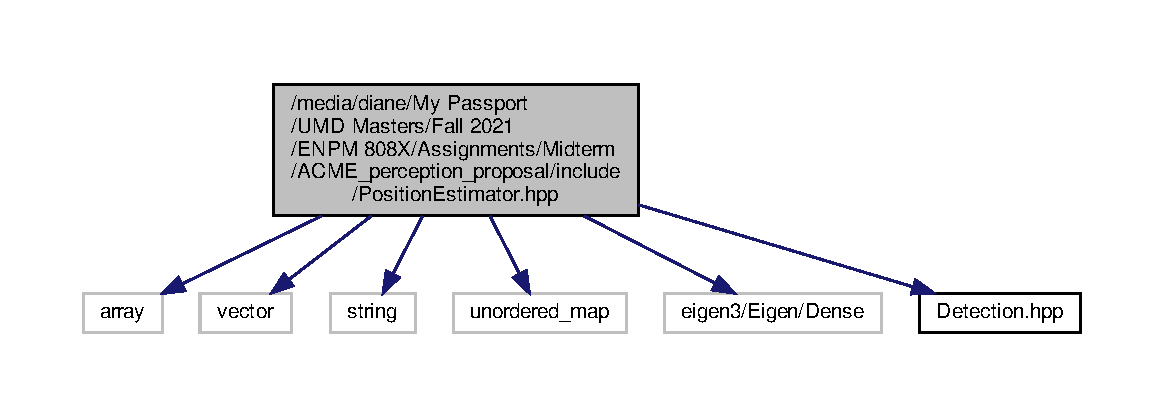
\includegraphics[width=350pt]{_position_estimator_8hpp__incl}
\end{center}
\end{figure}
This graph shows which files directly or indirectly include this file\+:
\nopagebreak
\begin{figure}[H]
\begin{center}
\leavevmode
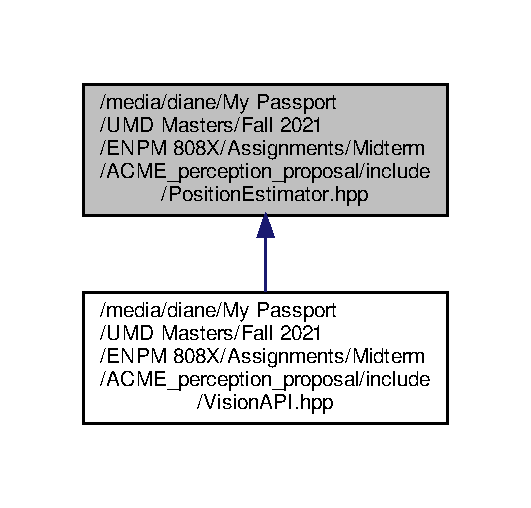
\includegraphics[width=255pt]{_position_estimator_8hpp__dep__incl}
\end{center}
\end{figure}
\subsection*{Classes}
\begin{DoxyCompactItemize}
\item 
class \hyperlink{class_position_estimator}{Position\+Estimator}
\end{DoxyCompactItemize}

\hypertarget{utils_8hpp}{}\section{/media/diane/\+My Passport/\+U\+MD Masters/\+Fall 2021/\+E\+N\+PM 808\+X/\+Assignments/\+Midterm/\+A\+C\+M\+E\+\_\+perception\+\_\+proposal/include/utils.hpp File Reference}
\label{utils_8hpp}\index{/media/diane/\+My Passport/\+U\+M\+D Masters/\+Fall 2021/\+E\+N\+P\+M 808\+X/\+Assignments/\+Midterm/\+A\+C\+M\+E\+\_\+perception\+\_\+proposal/include/utils.\+hpp@{/media/diane/\+My Passport/\+U\+M\+D Masters/\+Fall 2021/\+E\+N\+P\+M 808\+X/\+Assignments/\+Midterm/\+A\+C\+M\+E\+\_\+perception\+\_\+proposal/include/utils.\+hpp}}


utils header  


{\ttfamily \#include $<$string$>$}\newline
{\ttfamily \#include $<$vector$>$}\newline
{\ttfamily \#include $<$stdexcept$>$}\newline
Include dependency graph for utils.\+hpp\+:
\nopagebreak
\begin{figure}[H]
\begin{center}
\leavevmode
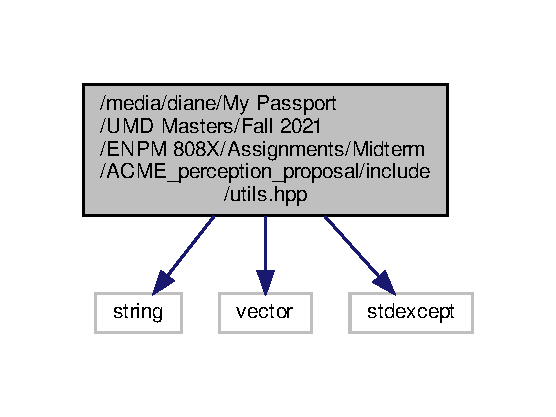
\includegraphics[width=267pt]{utils_8hpp__incl}
\end{center}
\end{figure}
\subsection*{Classes}
\begin{DoxyCompactItemize}
\item 
class \hyperlink{class_invalid_file}{Invalid\+File}
\begin{DoxyCompactList}\small\item\em \hyperlink{class_invalid_file}{Invalid\+File} exception for parsers. \end{DoxyCompactList}\end{DoxyCompactItemize}
\subsection*{Functions}
\begin{DoxyCompactItemize}
\item 
{\footnotesize template$<$typename Out $>$ }\\void \hyperlink{utils_8hpp_a03529396588a5d4dac36c432989fdfaa}{split} (const std\+::string \&s, char delim, Out result)
\begin{DoxyCompactList}\small\item\em Splits a string into a series of alpha-\/numeric words. \end{DoxyCompactList}\item 
std\+::vector$<$ std\+::string $>$ \hyperlink{utils_8hpp_a6462346f3d490257a819c0a4f17de83a}{split} (const std\+::string \&s, char delim=\textquotesingle{} \textquotesingle{})
\begin{DoxyCompactList}\small\item\em Splits string by the delimeter and returns a vector. \end{DoxyCompactList}\end{DoxyCompactItemize}


\subsection{Detailed Description}
utils header 

\begin{DoxyAuthor}{Author}
Dani Lerner 

Diane Ngo 
\end{DoxyAuthor}
\begin{DoxyVersion}{Version}
0.\+1 
\end{DoxyVersion}
\begin{DoxyDate}{Date}
2021-\/10-\/25
\end{DoxyDate}
\begin{DoxyCopyright}{Copyright}
Copyright (c) 2021 
\end{DoxyCopyright}


\subsection{Function Documentation}
\mbox{\Hypertarget{utils_8hpp_a03529396588a5d4dac36c432989fdfaa}\label{utils_8hpp_a03529396588a5d4dac36c432989fdfaa}} 
\index{utils.\+hpp@{utils.\+hpp}!split@{split}}
\index{split@{split}!utils.\+hpp@{utils.\+hpp}}
\subsubsection{\texorpdfstring{split()}{split()}\hspace{0.1cm}{\footnotesize\ttfamily [1/2]}}
{\footnotesize\ttfamily template$<$typename Out $>$ \\
void split (\begin{DoxyParamCaption}\item[{const std\+::string \&}]{s,  }\item[{char}]{delim,  }\item[{Out}]{result }\end{DoxyParamCaption})}



Splits a string into a series of alpha-\/numeric words. 

{\bfseries [https\+://stackoverflow.\+com/questions/236129/how-\/do-\/i-\/iterate-\/over-\/the-\/words-\/of-\/a-\/string]}


\begin{DoxyParams}{Parameters}
{\em input} & \\
\hline
\end{DoxyParams}
\begin{DoxyReturn}{Returns}
Changes \char`\"{}out\char`\"{} container 
\end{DoxyReturn}
\mbox{\Hypertarget{utils_8hpp_a6462346f3d490257a819c0a4f17de83a}\label{utils_8hpp_a6462346f3d490257a819c0a4f17de83a}} 
\index{utils.\+hpp@{utils.\+hpp}!split@{split}}
\index{split@{split}!utils.\+hpp@{utils.\+hpp}}
\subsubsection{\texorpdfstring{split()}{split()}\hspace{0.1cm}{\footnotesize\ttfamily [2/2]}}
{\footnotesize\ttfamily std\+::vector$<$std\+::string$>$ split (\begin{DoxyParamCaption}\item[{const std\+::string \&}]{s,  }\item[{char}]{delim = {\ttfamily \textquotesingle{}~\textquotesingle{}} }\end{DoxyParamCaption})}



Splits string by the delimeter and returns a vector. 


\begin{DoxyParams}{Parameters}
{\em s} & \\
\hline
{\em delim} & \\
\hline
\end{DoxyParams}
\begin{DoxyReturn}{Returns}
std\+::vector$<$std\+::string$>$ 
\end{DoxyReturn}

\hypertarget{_vision_a_p_i_8hpp}{}\section{/media/diane/\+My Passport/\+U\+MD Masters/\+Fall 2021/\+E\+N\+PM 808\+X/\+Assignments/\+Midterm/\+A\+C\+M\+E\+\_\+perception\+\_\+proposal/include/\+Vision\+A\+PI.hpp File Reference}
\label{_vision_a_p_i_8hpp}\index{/media/diane/\+My Passport/\+U\+M\+D Masters/\+Fall 2021/\+E\+N\+P\+M 808\+X/\+Assignments/\+Midterm/\+A\+C\+M\+E\+\_\+perception\+\_\+proposal/include/\+Vision\+A\+P\+I.\+hpp@{/media/diane/\+My Passport/\+U\+M\+D Masters/\+Fall 2021/\+E\+N\+P\+M 808\+X/\+Assignments/\+Midterm/\+A\+C\+M\+E\+\_\+perception\+\_\+proposal/include/\+Vision\+A\+P\+I.\+hpp}}


Vision A\+PI header.  


{\ttfamily \#include $<$array$>$}\newline
{\ttfamily \#include $<$vector$>$}\newline
{\ttfamily \#include $<$string$>$}\newline
{\ttfamily \#include $<$memory$>$}\newline
{\ttfamily \#include $<$unordered\+\_\+map$>$}\newline
{\ttfamily \#include $<$opencv2/opencv.\+hpp$>$}\newline
{\ttfamily \#include \char`\"{}./\+Human\+Detector.\+hpp\char`\"{}}\newline
{\ttfamily \#include \char`\"{}./\+Position\+Estimator.\+hpp\char`\"{}}\newline
{\ttfamily \#include \char`\"{}./\+Detection.\+hpp\char`\"{}}\newline
Include dependency graph for Vision\+A\+P\+I.\+hpp\+:
\nopagebreak
\begin{figure}[H]
\begin{center}
\leavevmode
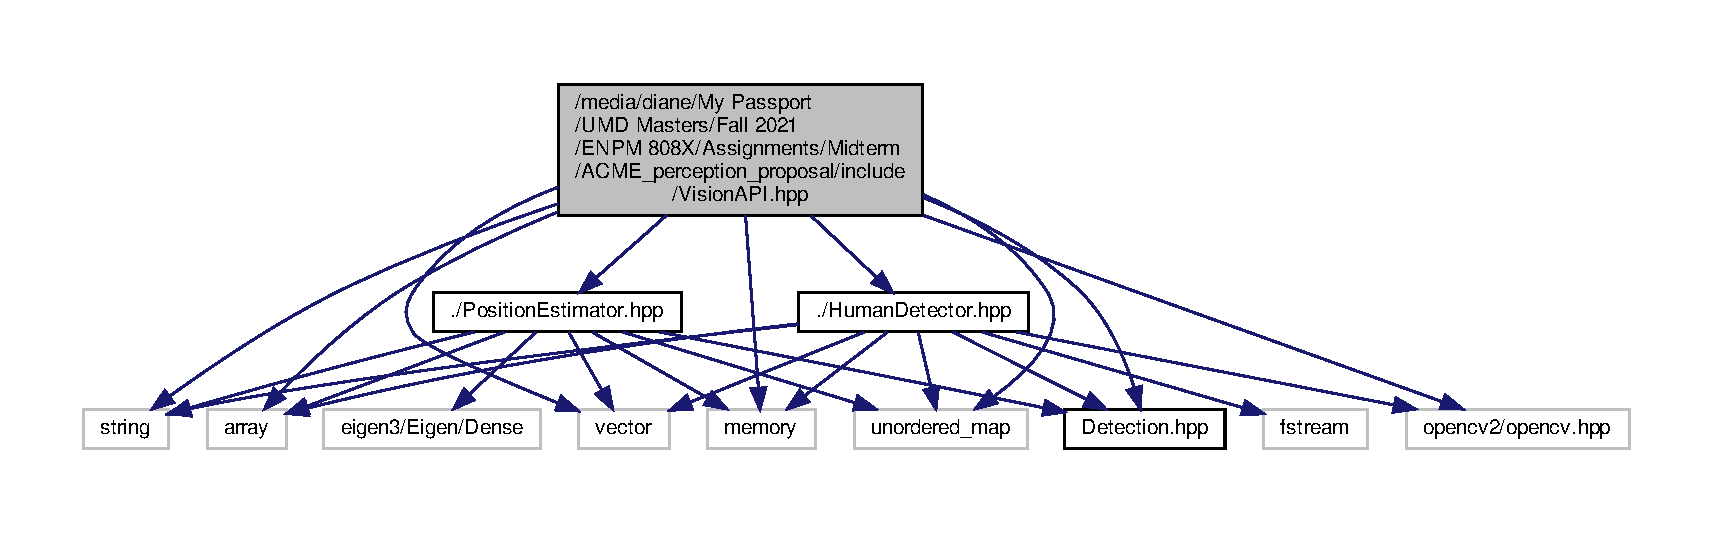
\includegraphics[width=350pt]{_vision_a_p_i_8hpp__incl}
\end{center}
\end{figure}
\subsection*{Classes}
\begin{DoxyCompactItemize}
\item 
class \hyperlink{class_vision_a_p_i}{Vision\+A\+PI}
\end{DoxyCompactItemize}


\subsection{Detailed Description}
Vision A\+PI header. 

\begin{DoxyAuthor}{Author}
Dani Lerner 

Diane Ngo 
\end{DoxyAuthor}
\begin{DoxyVersion}{Version}
0.\+1 
\end{DoxyVersion}
\begin{DoxyDate}{Date}
2021-\/10-\/25
\end{DoxyDate}
\begin{DoxyCopyright}{Copyright}
Copyright (c) 2021 
\end{DoxyCopyright}

%--- End generated contents ---

% Bibliography
\newpage
\phantomsection
\bibliographystyle{plain}
\bibliography{}
\addcontentsline{toc}{chapter}{Bibliography}

% Index
\backmatter
\newpage
\phantomsection
\clearemptydoublepage
\addcontentsline{toc}{chapter}{Index}
\printindex

\end{document}
